\documentclass{standalone}
\usepackage{tikzducks}

\begin{document}
	
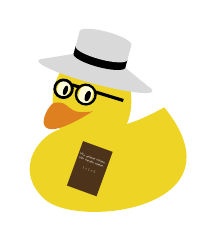
\begin{tikzpicture}
	\duck[glasses,
	bookcolour=black!60!brown,
	book={
			\scalebox{0.14}{
			\parbox{2.5cm}{
			\sffamily
			\centering
			\footnotesize
	    Wir m\"ussen wissen.\\
	    Wir werden wissen.\\[0.4cm]
	    $1+1=2$}}}
	]
  \fill[gray!30!white,rotate=-15] (0.44,2.0) ellipse (0.75 and 0.1);  
  \fill[gray!30!white,rotate=-15] (0.1,2.05) rectangle (0.78,2.5);
  \fill[gray!30!white,rotate=-15] (0.44,2.5) ellipse (0.34 and 0.08);  
  \fill[gray!30!white,rotate=-15] (-0.3,2.02) -- (1.18,2.02) -- (0.78,2.2) -- (0.1,2.2) -- cycle;
  \fill[black,rotate=-15] (0.44,2.2) ellipse (0.34 and 0.08);   
  \fill[black,rotate=-15] (0.1,2.2) rectangle (0.78,2.3);
	\fill[gray!30!white,rotate=-15] (0.44,2.3) ellipse (0.34 and 0.08);  

\end{tikzpicture}	
	
\end{document}